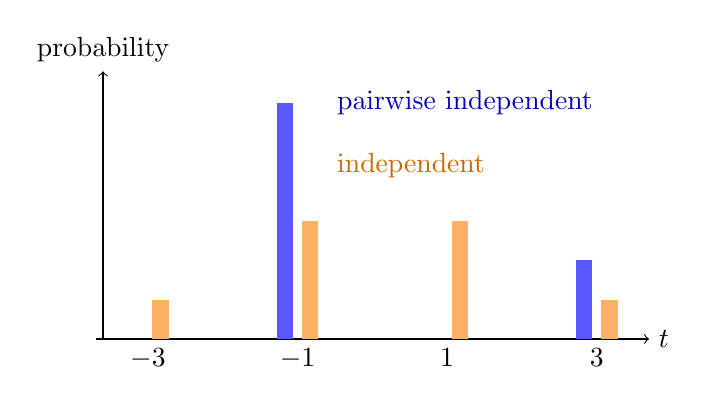
\begin{tikzpicture}[x=.95cm,y=4cm]
\draw[->] (-3.7,0)--(3.7,0) node[right] {$t$};
\draw[->] (-3.6,0)--(-3.6,.85) node[above] {probability};
\foreach \x/\y in {-3/.125,-1/.375,1/.375,3/.125}{\fill[orange!60] (\x+.06,0) rectangle (\x+.28,\y);}
\foreach \x/\y in {-1/.75,3/.25}{\fill[blue!65] (\x-.28,0) rectangle (\x-.06,\y);}
\foreach \x in {-3,-1,1,3}{\node[below] at (\x,0) {$\x$};}
\node[blue!70!black,anchor=west] at (-.6,.75) {pairwise independent};
\node[orange!80!black,anchor=west] at (-.6,.55) {independent};
\end{tikzpicture}
